
{\pubs} is a data processing software framework that supports a specific
data process model implementation by application developers. In particular,
it has following features:
\begin{itemize}
  \item Use {\psql} for process management
  \item Supports {\python} code development for implementation
  \item Provides {\php} toolkit for application management and monitoring
\end{itemize}
This section describes a generic idea of {\pubs} data processing model.

\subsection{Project: A Unit Task of Data Processing}
\label{pubs:model:project}
A typical model of data processing is a well defined chain of processes
in which a particular process is triggered by a completion or an initiation
of another process. For instance, the end of running DAQ may trigger a file
transfer protocole to move a raw data file to a storage server. In {\pubs},
each of such processes is called a {\it project}. 

\subsubsection{Project Status}
Each {\pubs} project carries a specific {\it status} code represented
by an integer. A unit of status is defined by, in case of MicroBooNE, a
unique combination of four integeres: run, sub-run, {\it sequence} 
(or simply {\it seq}), and the project version number. This combination is
referred to as {\it TaskID} in this document. A run and sub-run numbers 
defines a boundary of data taking  defined by a DAQ as you might guess. 
A sequence number, on the other hand, is a possible sub-set of run and 
sub-run number combination, and is defined by a project. It is there to 
support some projects that may need to sub-divide a process to deal with 
a particular DAQ run. As its name says, the project version is an integer
representing different version of the same project. 

Each {\pubs} project carries a status for each TaskID. Special status code 
1 is reserved to represent the initial status for any project. Similarly, 
code 0 is reserved to represent the completion status for any 
project. Any other integer values may be used to represent various status 
which meaning may be defined by a project.

\subsubsection{Project Version}
One important feature of data processing framework is an ability to roll-back
and re-process some older data files. Reprocessing of data is supported in
{\pubs}, but it requires to change a project version number. The basic 
assumption for forcing the version update for re-processing is that something
must have changed to roll back and re-process data. 
\begin{figure}[ht]\begin{center}
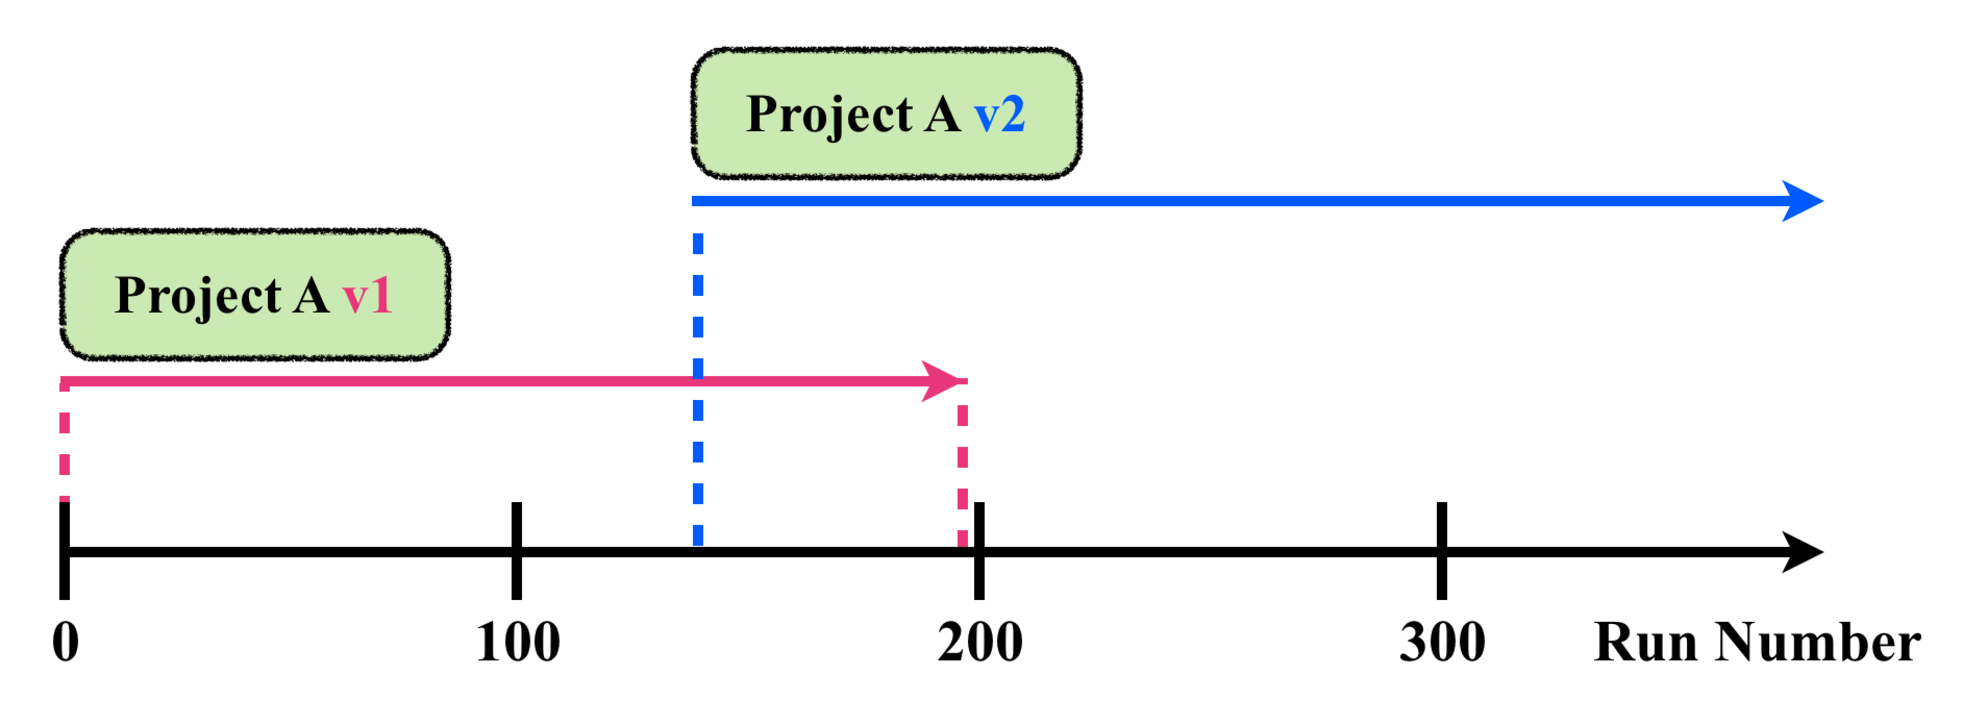
\includegraphics[width=14cm]{./img/PUB_ProjectVersion.pdf}
\caption{ Example diagram showing how project version may be used. 
The horizontal axis shows the time in the unit of a run number 
(sub-run number ignored for simplicity). The diagram shows that the 1st 
version of project A processing data up to around run 200. Then the updated 
2nd version starts re-processing runs just before around run 150 and takes 
over to process all future runs.}
\label{pubs:model:version}
\end{center}\end{figure}
Figure\ref{pubs:model:version} shows an example of reprocessing associated
with a specific project's version update.


\subsubsection{Project Table}
Each project status is stored in {\psql} database table with a name same
as the project's name, called a project table. For this reason, {\bf a 
project name must be unique}. A project table contains several information 
per unique combination of run, sub-run, seq numbers, and they are shown below 
with corresponding {\psql} data type.
\begin{itemize}
\item Run $\ldots$ INT $\ldots$ DAQ run number
\item SubRun $\ldots$ INT $\ldots$ DAQ sub-run number
\item Seq $\ldots$ SMALLINT $\ldots$ project sequence number
\item Status $\ldots$ SMALLINT $\ldots$ project status code
\item Data $\ldots$ TEXT $\ldots$ Generic ``data'' associated with a particular run, sub-run combination
\item ProjectVer $\ldots$ SMALLINT $\ldots$ a version number for a project
\end{itemize}
A project may record some ``data'' in string representation for each TaskID.
However, it is recommended to avoid to store such information when possible 
as this makes the table size to become larger. Finally, as mentioned before,
a project is allowed to have a different version number. 

\subsubsection{Project Execution Model}
Each project is expected to have a single {\python} script to be executed.
This {\python} script should fetch an array of target TaskID from the 
database based on a status code. Depending on the status code, then, the
script may take a certain action, and possibly update the status code in the
database upon success. In short, the status code is used as a trigger for
a specific action by projects. 

Now, information needed to execute each such script is called {\it project
information}, and is stored in a separate database table called the 
{\it ProcessTable}. In the next section, we discuss about this table and
also a machinary to automatically execute a project's {\python} script
using a daemon tool.

\subsection{ProcessTable And Daemon Execution}
\label{pubs:model:daemon}
Information about individual project is stored in a dedicated database
table called ``ProcessTable''. Unlike project tables that exist one per
project, this is a unique table in the database that holds all projects'
information. The table schema is shown below:
\begin{itemize}
  \item ID $\ldots$ SERIAL $\ldots$ a unique integer key for each project
  \item Project $\ldots$ TEXT $\ldots$ the name of a project
  \item ProjectVer $\ldots$ SMALLINT $\dots$ the version number of a project
  \item Command $\ldots$ TEXT $\ldots$ a project execution command to be run
  \item Frequency $\ldots$ INT $\ldots$ latency in seconds between each execution of a project
  \item EMail $\ldots$ TEXT $\ldots$ email contact(s) in case of a trouble
  \item StartRun $\ldots$ INT $\ldots$ the first run-number to be processed
  \item StartSubRun $\ldots$ INT $\ldots$ the first sub-run number to be processed
  \item Resource $\ldots$ HSTORE $\ldots$ a dynamic string-to-string map data container
  \item Enabled $\ldots$ BOOLEAN $\ldots$ a boolean flag for project execution (only if it is true)
  \item Running $\ldots$ BOOLEAN $\ldots$ a boolean flag enabled during project execution
  \item LogTime $\ldots$ TIMESTAMP $\ldots$ a time-stamp logged per entry update
\end{itemize}
where, among many self-descriptive columns, ``Resource'' column holds HSTORE
type variable that can be used to store any project-specific information.
Such information includes, for example, the path to a specific data directory
and expected file name format that requires run and sub-run numbers such as
\begin{center}
 {\ttfamily Run\%05d\_SubRun\%03d.bin}.
\end{center}
with which your project can figure out the expected file name for a given
TaskID (i.e. run and sub-run numbers). 

Note that storing such information in ProcessTable is much lighter than 
storing the actual filename in a project table's ``Data'' column because 
the ``Data'' column stores information for every single TaskID while 
ProcessTable entry is made only one per project. Again, store as much
information as possible in ProcessTable and avoid using ``Data'' column
of a project table when possible.

\subsubsection{Daemon: Master Scheduler}
An execution of a project should be as simple as:
\begin{lstlisting}
  > python my_project.py
\end{lstlisting}
where my\_project.py is the executor of a project. In {\pubs}, however,
there is a simple daemon project management tool that periodically 
looks up the ProcessTable and executes the enabled projects in parallel. 
So it is a lot like {\ttfamily cron} in Unix/Linux but with a process
manager aspect.  

The daemon process is responsible for project management: it keeps track
of history of running each project, and it ensures its resoure usage. 
The project information is updated every 120 seconds (configurable) and 
synchronized with the ProcessTable contents in the database. An expert
can impose a change in project information without interrupting the daemon
process. Another important role of the daemon is to keep the integrity of
the DAQ's run table with all enabled projects' table. Once in every 300
seconds (configurable), the daemon process synchronizes run and sub-run
number entries in each project table and match with the DAQ run table.

That being said, it is extremely important that each project is a truly
modulated action, and does not depend on an execution by the daemon. In
other words, one should be able to always run a project by simply invoking
from a command line. This allows us to take any emergency treatment when,
somehow, the daemon procedure cannot be used.

\begin{figure}\begin{center}
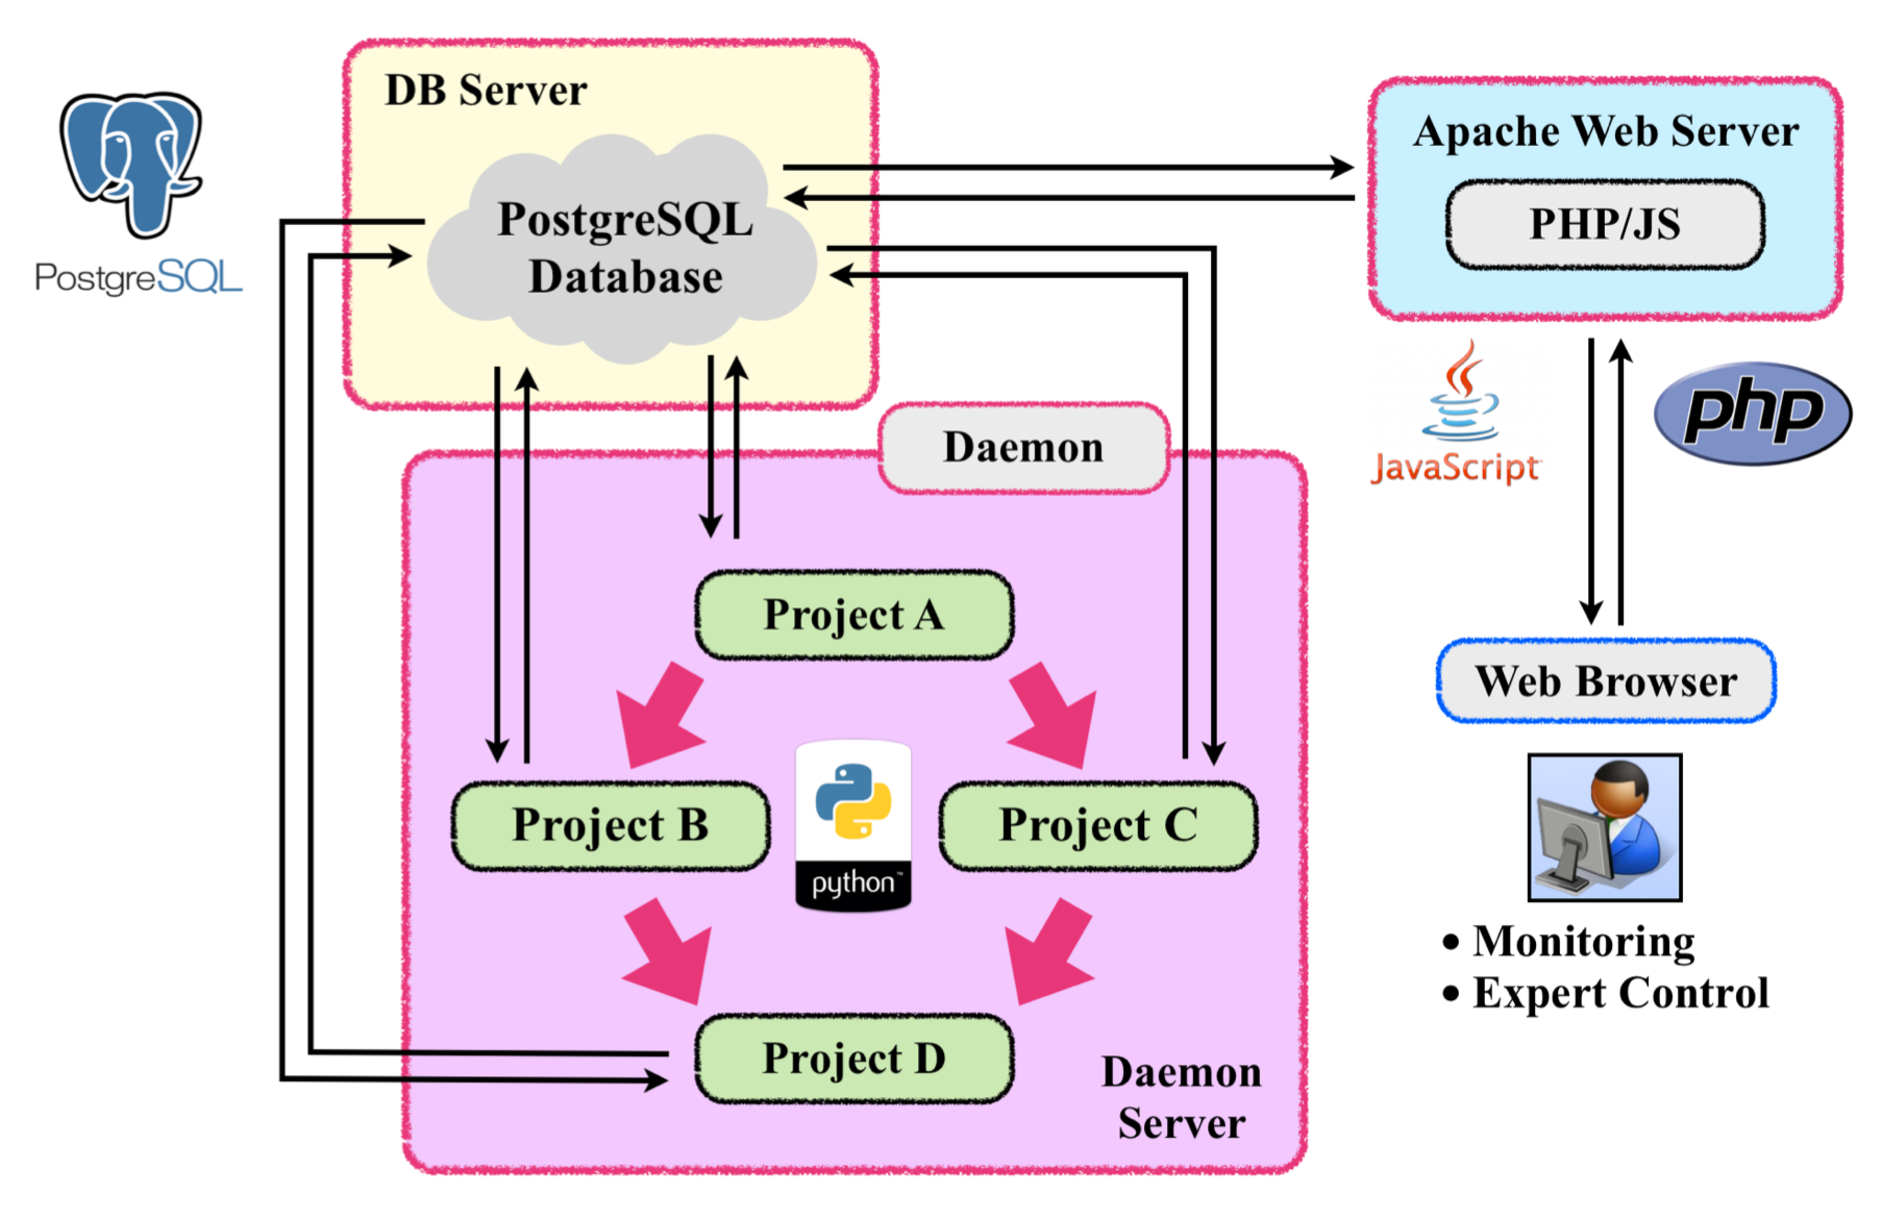
\includegraphics[width=14.5cm]{./img/PUB_Model.pdf}
\caption{ An abstract drawing that shows how data flows into and from the
{\psql} database within {\pubs} framework. Each project and daemon process
all talk to the database server. The {\php} web-interface provides monitoring
and project management tools.}
\label{pubs:model:model}
\end{center}\end{figure}


\subsection{Web Monitoring And Process Management}
\label{pubs:model:monitor}

Figure\ref{pubs:model:model} shows a brief data flow from and into the 
{\psql} database. As described in Sec.\ref{pubs:model:project} and
\ref{pubs:model:daemon}, each project and daemon accesses the database
server individually. In addition to the project execution framework, 
{\pubs} provides {\php} based monitoring and management interface through 
a web server machine and end-user's web browser application. Accordingly
there is a database connection between the web server and {\psql} server
machines.

The capability to monitor each projects' status through a web browser is
quite useful for a routine inspection, such as shifters' check list.
Similarly a formatted control pannel for managing project
execution is useful for experts to take action without logging into the
machine. The details of {\php} implementation is quite experiment specific, 
and the MicroBooNE usage will be discussed in Ch.\ref{dstream}. 
